\chapter{Aplicación}
    \section{Requisitos}
        \begin{itemize}
            \item Conexión a WiFi.
            \item Encontrarse cerca de la batería.
            \item Celular Android.
            \item Versión de Android 11 o superior.
            \item Espacio de 10 MB (Megabytes) en su celular.
        \end{itemize}

    \section{Guía de Instalación}
       Para descargar la aplicación en su dispositivo móvil, deberá ingresar desde su celular a nuestro repositorio de github, más concretamente hacia la parte de la app. Puede ir directo hacia allá con el siguiente link:\par
       
       \vspace{0.5cm}
       
       \begin{center}
           \href{https://github.com/impatrq/gravicap/tree/main/GraviCap_app/Instalacion%20de%20la%20Aplicacion%20Movil}{https://github.com/impatrq/gravicap/tree/main/GraviCap\_app/Instalacion\%20de\%20la\%20Aplicacion\%20Movil}\par
       \end{center}

        \vspace{0.5cm}
        
        Una vez ingresemos al link, veremos los siguientes archivos:\par
        
        \begin{figure} [H]
            \centering
            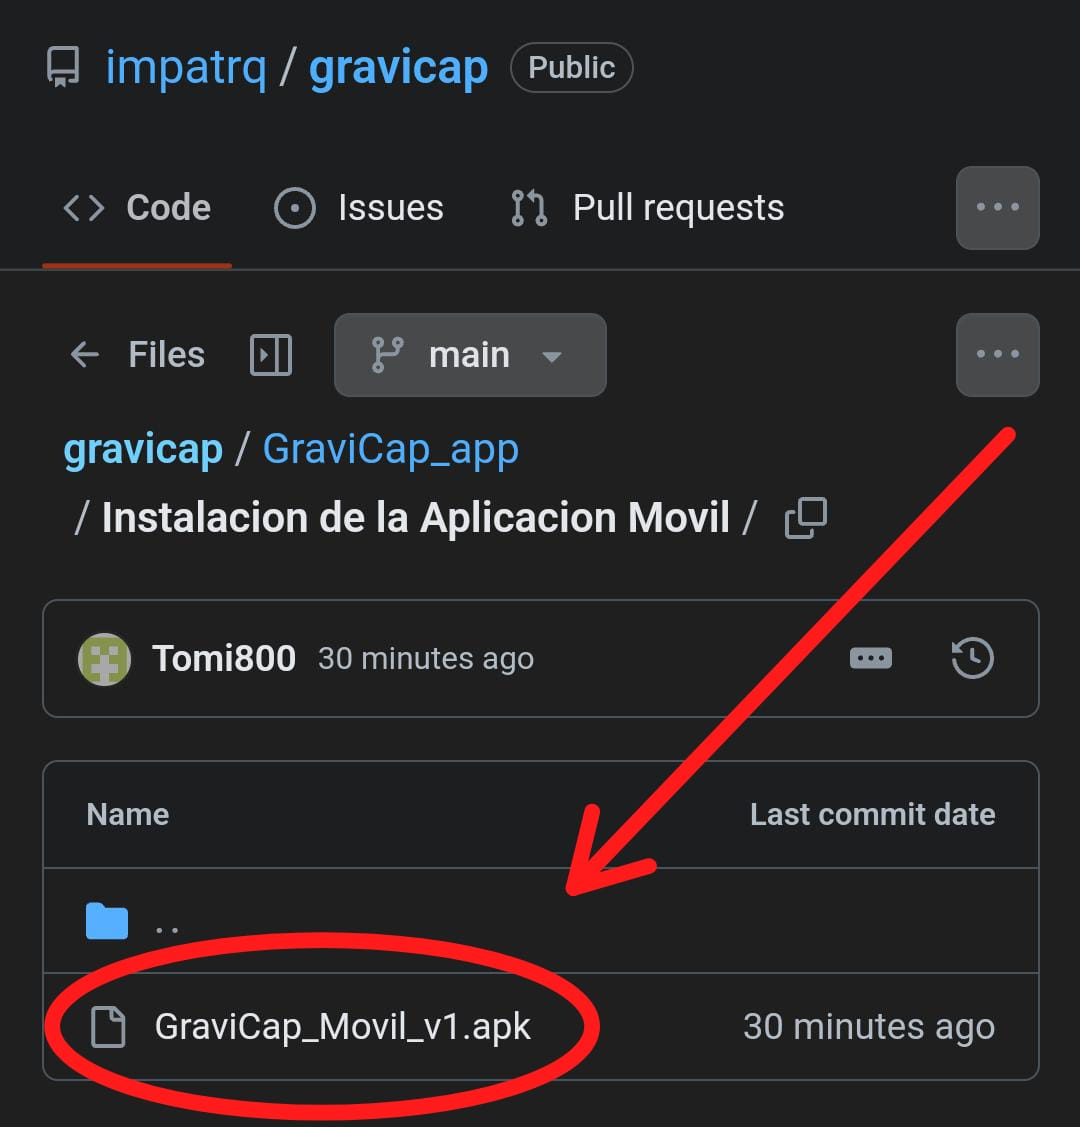
\includegraphics[width=0.5\linewidth]{Imagenes/Aplicacion/I1.png}
        \end{figure}
        
        Ingresamos al archivo indicado, el cual es el .apk de la aplicación, el archivo ejecutable para poder descargar la aplicación desde el celular. También podremos encontrar otros archivos .apk, los cuales son las diferentes versiones de la app.\par

        \begin{figure} [H]
            \centering
            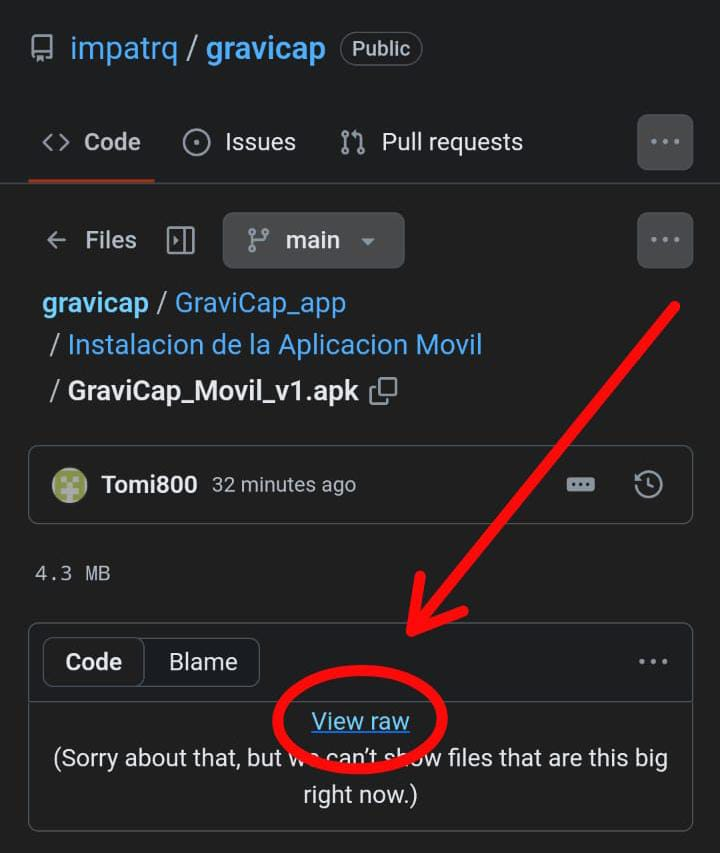
\includegraphics[width=0.5\linewidth]{Imagenes/Aplicacion/I2.png}
        \end{figure}

        Presionaremos el botón de “view raw” para descargar la aplicación.\par

        \begin{figure} [H]
            \centering
            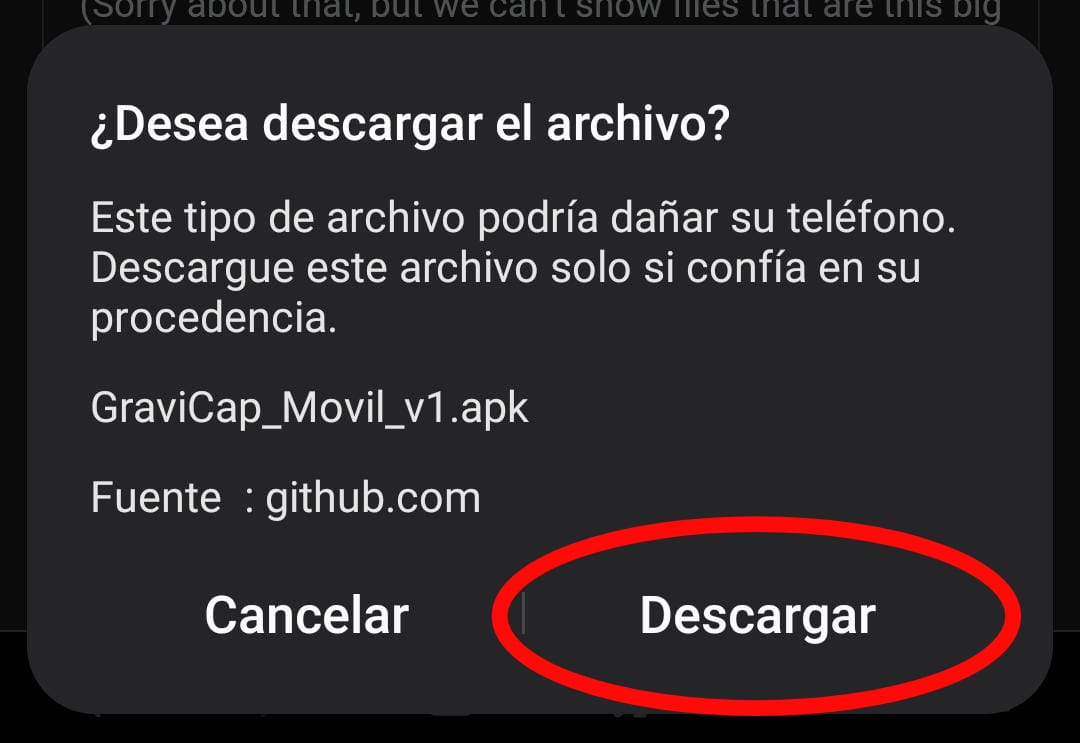
\includegraphics[width=0.5\linewidth]{Imagenes/Aplicacion/I3.png}
        \end{figure}

        Finalmente, reconocerá que se quiere descargar la aplicación, solamente presionamos el botón de “descargar” y comenzará la descarga de la aplicación.\par
        También puede que dependiendo de su sistema operativo y celular, requiera de aceptar la descarga nuevamente.\par
        Una vez descargada, podrá ingresar directamente y podrá ver la aplicación en su celular de esta manera.\par

        \begin{figure} [H]
            \centering
            
\includegraphics[width=0.5\linewidth]{Imagenes/Aplicacion/I4.png}
        \end{figure}
        \begin{center}
            \Large{\textbf{¡Felicidades, ya puede utilizar la aplicación de \textcolor{dark_violet}{GraviCap}!}}\par
        \end{center}
        
        \newpage
    \section{Bienvenida}
        Cada usuario, al ingresar a la aplicación, verá nuestro logo con su respectivo nombre, y slogan.\par

        \begin{figure} [H]
            \centering
            
\includegraphics[width=0.5\linewidth]{Imagenes/Aplicacion/1.png}
        \end{figure}

        También encontrará un texto que le proveerá una pequeña información de nuestro producto, los valores de la batería que podrá monitorear, así también como gráficos lineales en base a valores registrados de la batería.\par

        \begin{figure} [H]
            \centering
            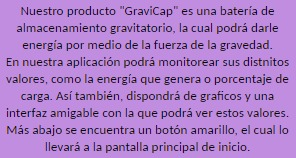
\includegraphics[width=0.5\linewidth]{Imagenes/Aplicacion/2.png}
        \end{figure}

        Una vez el usuario haya leído el texto, encontrará en la parte inferior de la pantalla un botón amarillo con texto “Pulse Aquí para ir a Inicio” el cual lo llevará hacia la pantalla de principal de Inicio para poder navegar por las diferentes pantallas y ver los valores de la batería.\par

        \begin{figure} [H]
            \centering
            
\includegraphics[width=0.5\linewidth]{Imagenes/Aplicacion/3.png}
        \end{figure}

        \begin{figure} [H]
            \centering
            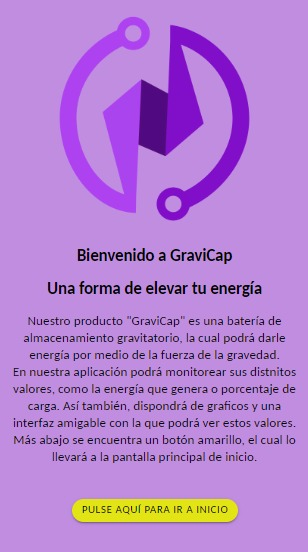
\includegraphics[width=0.5\linewidth]{Imagenes/Aplicacion/4.png}
        \end{figure}

    \section{Inicio}
        Al pulsar el botón de la pantalla de bienvenida, se encontrará con la pantalla principal, la pantalla de inicio. Teniendo en cuenta la navegación del usuario por los diferentes valores, situamos los botones pensando en un recorrido eficiente, intuitivo y amigable para el mismo.\par
        La primera parte que verá el usuario, será una barra blanca en la parte superior (header), contando con nuestro logo en la parte izquierda, un texto amigable de bienvenida en la parte central y un botón de información en la parte izquierda, el cual, contiene nuestras redes y contactos.

        \begin{figure} [H]
            \centering
            
\includegraphics[width=0.5\linewidth]{Imagenes/Aplicacion/5.png}
        \end{figure}

        \begin{figure} [H]
            \centering
            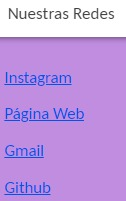
\includegraphics[width=0.5\linewidth]{Imagenes/Aplicacion/6.png}
        \end{figure}

        En la parte central de la pantalla, el usuario podrá ver su contenido principal, conformado por botones con imágenes y textos referenciados al valor que podrá monitorear.\par
        Estos están ubicados de forma tal que el usuario pueda ver y entrar a las pantallas de los valores importantes con mayor comodidad.\par
        Los dos botones ubicados en la parte de arriba son los valores más importantes y la sección de los tres botones en la parte inferior no serán de primordial importancia para el usuario. Algunos de estos valores son: la energía que genera la batería; su carga; el consumo que tiene el usuario; los valores del panel solar y valores generales de la batería.\par

        \begin{figure} [H]
            \centering
            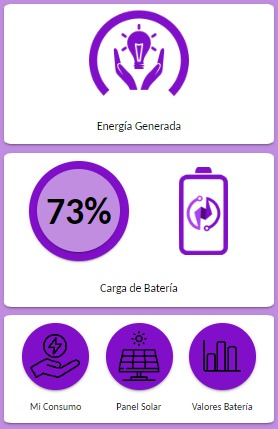
\includegraphics[width=0.5\linewidth]{Imagenes/Aplicacion/7.png}
        \end{figure}

        En la parte inferior izquierda encontraremos un pequeño botón amarillo con texto “Página de Gráficos” el cual, nos enviará a una pantalla en la cual podremos ver los distnitos tipos de gráficos de potencia de la batería.\par

        \begin{figure} [H]
            \centering
            
\includegraphics[width=0.5\linewidth]{Imagenes/Aplicacion/8.png}
        \end{figure}

        \begin{figure} [H]
            \centering
            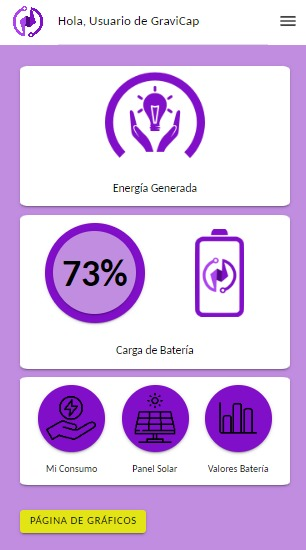
\includegraphics[width=0.5\linewidth]{Imagenes/Aplicacion/9.png}
        \end{figure}

    \section{Paginas y Valores}
        Todas las pantallas cuentan con una barra blanca (header) en la parte superior que contienen un botón para ir hacia atrás, es decir, que podrán volver a la pantalla principal de inicio.\par
        Una de las pantallas importantes que podrá ver el usuario es la de “Energía Generada”. El usuario, al entrar, verá un gráfico circular con el valor de potencia que tiene la batería. En la parte inferior podrán ver un texto referenciando el color del gráfico y el valor plasmado en la pantalla.\par

        \begin{figure} [H]
            \centering
            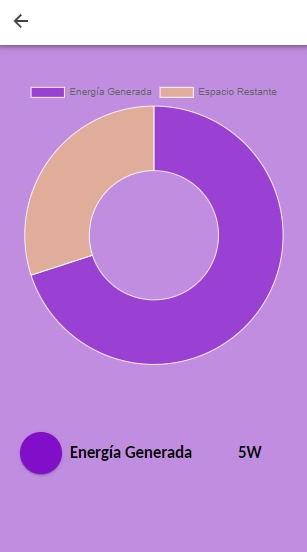
\includegraphics[width=0.5\linewidth]{Imagenes/Aplicacion/10.png}
        \end{figure}

        El usuario contará con la pantalla de “Carga de Batería” en la cual podrá ver un circulo de color violeta con un valor de carga porcentual, referenciando la carga que tiene la batería en ese momento, siendo el 100\% cuando el peso está en su punto más alto y el 0\% cuando el peso está en su punto más bajo. En la parte inferior el usuario podrá ver el tiempo que le falta a la batería para completar su carga.\par

        \begin{figure} [H]
            \centering
            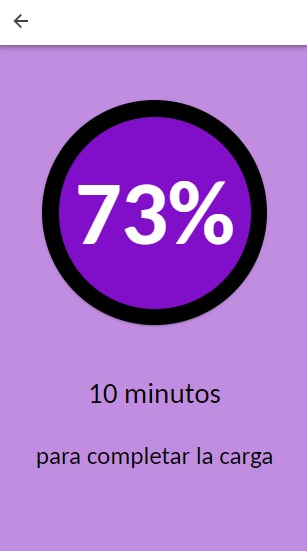
\includegraphics[width=0.5\linewidth]{Imagenes/Aplicacion/11.png}
        \end{figure}
        
        En la sección ubicada en la parte inferior podremos encontrar tres botones violetas con imágenes, referenciados a las pantallas de: consumo del usuario, valores del panel solar, valores generales de la batería.\par

        \begin{figure} [H]
            \centering
            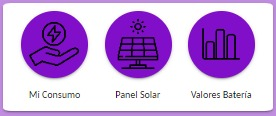
\includegraphics[width=0.5\linewidth]{Imagenes/Aplicacion/12.png}
        \end{figure}

        El usuario tendrá una pantalla dedicada para saber el consumo del dispositivo que esté cargando, esta pantalla será “Mi consumo”, esta pantalla contendrá una imagen de referencia del botón visto anteriormente y una carta con el texto “Su consumo es:” y el valor de potencia en watts.\par

        \begin{figure} [H]
            \centering
            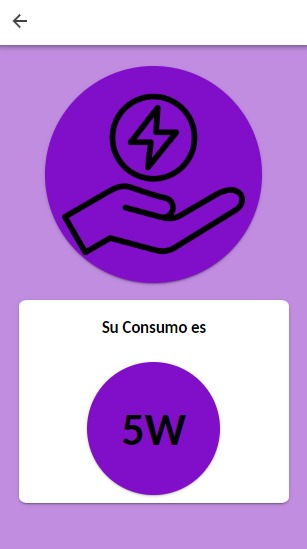
\includegraphics[width=0.5\linewidth]{Imagenes/Aplicacion/13.png}
        \end{figure}

        Para poder saber los valores del panel solar, el usuario dispone de la pantalla de “Panel Solar” en la cual podrá ver un circulo morado con una imagen de referencia del botón visto anteriormente y una carta con el texto “Valores del Panel Solar” y dos apartados: uno del voltaje con su respectivo valor en volts y el otro apartado de potencia con su respectivo valor en watts.\par

        \begin{figure} [H]
            \centering
            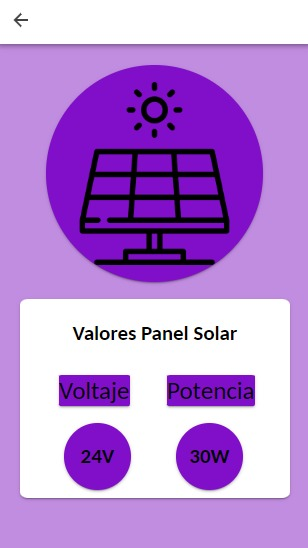
\includegraphics[width=0.5\linewidth]{Imagenes/Aplicacion/14.png}
        \end{figure}

        El último botón de la sección de tres le provee al usuario una información general de los “Valores de Batería”. Al ingresar en esta pantalla, el usuario verá un gráfico de tipo columnas referenciando 3 valores de la batería: voltaje, amperaje y wataje (potencia). En la parte inferior se podrá encontrar los valores numéricos de cada uno, referenciados con un círculo violeta y letras blancas.\par

        \begin{figure} [H]
            \centering
            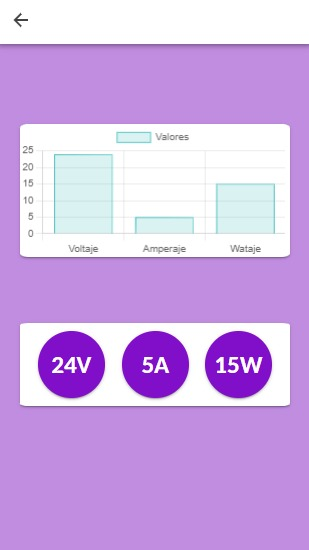
\includegraphics[width=0.5\linewidth]{Imagenes/Aplicacion/15.png}
        \end{figure}

    \section{Gráficos}
        Como se mencionó anteriormente, en la parte de la pantalla de inicio hay un botón que lleva al usuario a la pantalla de “Gráficos de la Batería”. Esta sección está creada para que el usuario pueda ver el funcionamiento de la batería en el momento de ascenso y descenso del peso, referenciado con valores de potencia en función del tiempo. El usuario, al entrar, verá una carta blanca con una imagen de gráfico con dos líneas, referenciando a los dos gráficos de potencia que podrá ver el usuario.\par

        \begin{figure} [H]
            \centering
            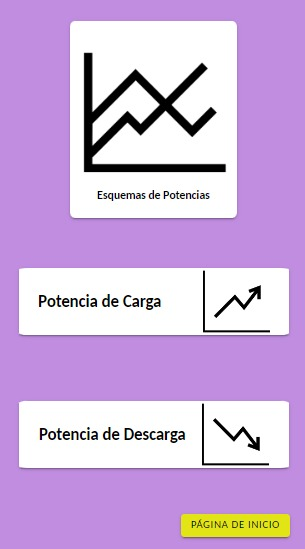
\includegraphics[width=0.5\linewidth]{Imagenes/Aplicacion/16.png}
        \end{figure}
        
        La parte central contiene dos botones, uno, el más de más arriba, con el texto “Potencia de Carga” con una imagen de un gráfico de línea ascendente.\par

        \begin{figure} [H]
            \centering
            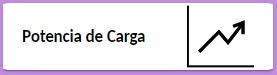
\includegraphics[width=0.5\linewidth]{Imagenes/Aplicacion/17.png}
        \end{figure}

        El botón de más abajo contiene el texto “Potencia de Descarga” con un gráfico de línea descendente.\par

        \begin{figure} [H]
            \centering
            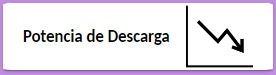
\includegraphics[width=0.5\linewidth]{Imagenes/Aplicacion/18.png}
        \end{figure}

        En la parte inferior de la página de gráficos el usuario verá un botón pequeño amarillo del mismo etilo que el de la pantalla de inicio, con el texto de “Página de Inicio” que al presionarlo lo llevará devuelta hacia la pantalla de inicio principal. \par

        \begin{figure} [H]
            \centering
            
\includegraphics[width=0.5\linewidth]{Imagenes/Aplicacion/19.png}
        \end{figure}

        Al presionar el botón con el icono de gráfico ascendente, el usuario podrá ver la pantalla de Potencia de Carga, esta es muy simple, únicamente encontrará el gráfico de línea ascendente de la batería, este se basa en la potencia que tiene la batería en el lapso de tiempo que este asciende, creando así un gráfico de potencia en función del tiempo.\par
        También, en la parte superior izquierda, encontramos un botón para volver atrás a la página de gráficos.\par

        \begin{figure} [H]
            \centering
            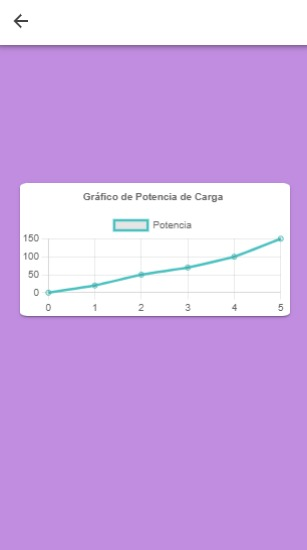
\includegraphics[width=0.5\linewidth]{Imagenes/Aplicacion/20.png}
        \end{figure}

        El segundo botón que contiene el icono de un gráfico descendente encontramos en la página de gráficos es el botón de Potencia de Descarga. Este actúa de igual forma que el botón mencionado anteriormente, únicamente que éste nos marcará el gráfico de potencia en función del tiempo cuando el peso esté en su momento de descenso.\par
        Este también cuenta con el botón para volver hacia atrás a la página de gráficos.\par

        \begin{figure} [H]
            \centering
            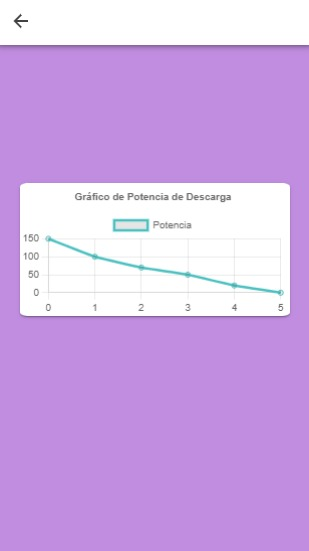
\includegraphics[width=0.5\linewidth]{Imagenes/Aplicacion/21.png}
        \end{figure}